After discovering Higgs boson\cite{HIGG-2012-27,CMS-HIG-12-028}, the examine of electroweak symmetry breaking (EWSB) becomes a main focus at the LHC.
In addition to measuring the properties of Higgs boson directly, the vector boson scattering (VBS) process is another key avenue to probe EWSB\cite{Lee:1977yc, Chanowitz:1985hj, Szleper:2014xxa}.
In Standard Model (SM), the Higgs boson acts as "moderator" to unitarize high-energy longitudinal VBS amplitudes at the TeV scale.
Therefore, studying high-energy behaviours of VBS is crucial to understand the mechanism of EWSB.

While no VBS process was observed prior to the LHC era, LHC provides an unexceptionable opportunity to study them due to its unprecedented high energy and lunimosity.
At LHC, the VBS process is typically studied through the measurements of electroweak (EW) production of two vector bosons radiated from initial-state quarks 
plus a pair hadronic jets with high energy in the back and forward regions (denoted as EW $VVjj$).
In the searches for EW $VVjj$ production, the quantum chromodynamics (QCD) production of $VVjj$, which contains two QCD vertices at the lowest order (denoted as QCD $VVjj$ processes), constitutes an irreducible background,
while it is part of signal in inclusive $VVjj$ cross section measurement in this talk.
The features of EW $VVjj$ production include a large invariant mass of jet pair ($m_{jj}$) and a significant separation of rapidity between two jets ($\Delta y_{jj}$).
Figure~\ref{fig:diagram} presents some typical Feynman diagrams of EW and QCD $ZZjj$ processes.
\begin{figure}[!htbp]
\begin{center}
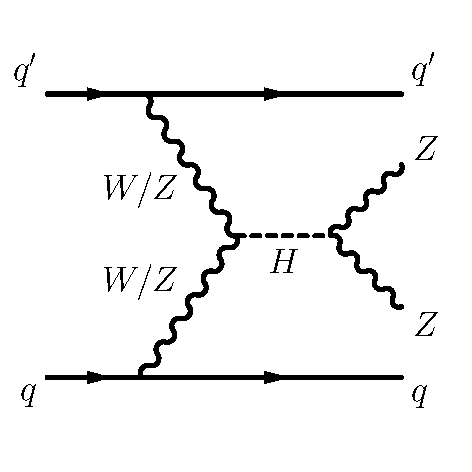
\includegraphics[width=0.22\textwidth]{figures/diagram/diagram-EWZZjj-Schn-Higgs.pdf}
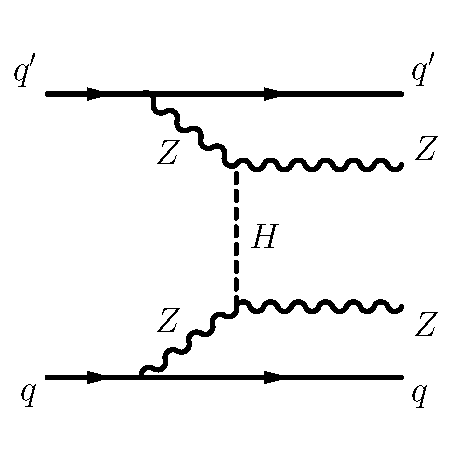
\includegraphics[width=0.22\textwidth]{figures/diagram/diagram-EWZZjj-Tchn-Higgs.pdf}
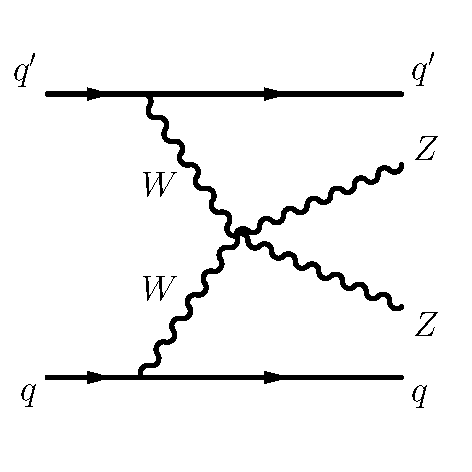
\includegraphics[width=0.22\textwidth]{figures/diagram/diagram-EWZZjj-QGC.pdf}
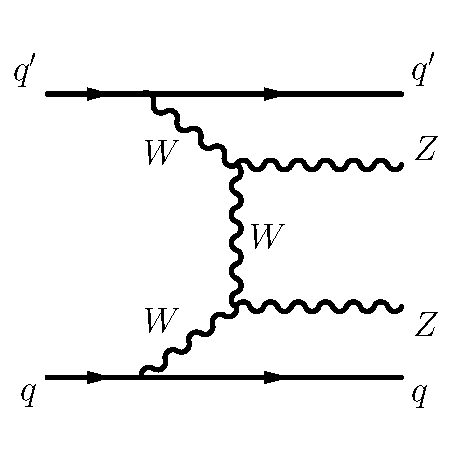
\includegraphics[width=0.22\textwidth]{figures/diagram/diagram-EWZZjj-TGC.pdf}\\
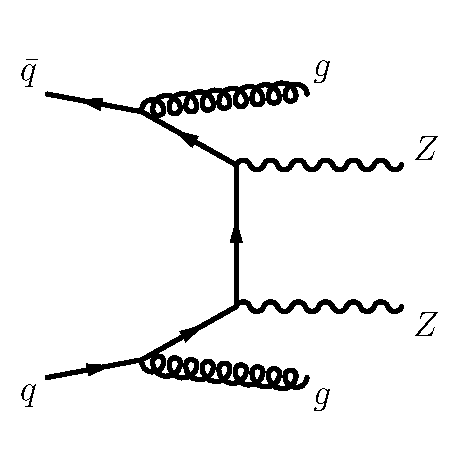
\includegraphics[width=0.22\textwidth]{figures/diagram/diagram-QCDZZjj-qq.pdf}
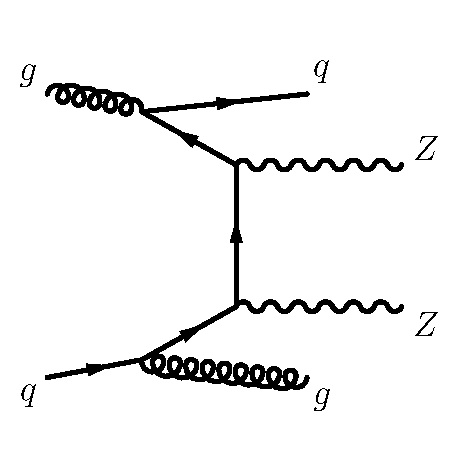
\includegraphics[width=0.22\textwidth]{figures/diagram/diagram-QCDZZjj-qg.pdf}
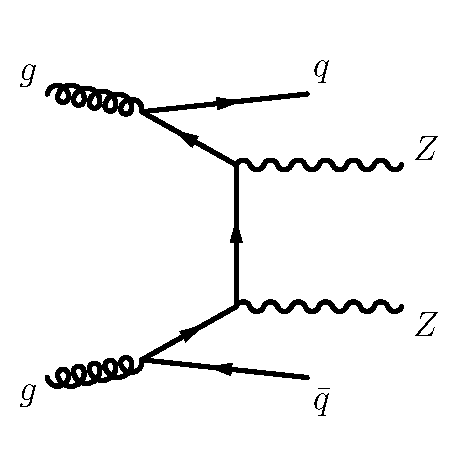
\includegraphics[width=0.22\textwidth]{figures/diagram/diagram-QCDZZjj-gg.pdf}
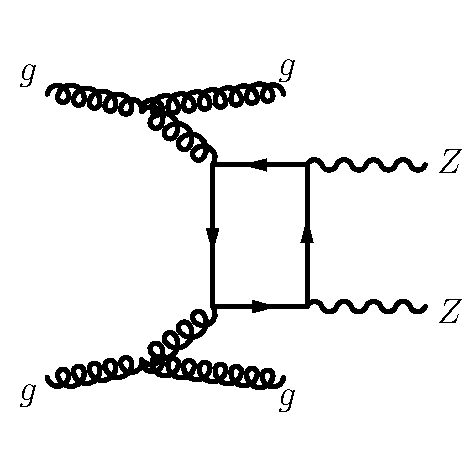
\includegraphics[width=0.22\textwidth]{figures/diagram/diagram-QCDZZjj-box.pdf}\\
\end{center}
\caption{Typical diagrams for the production of $ZZjj$, including the relevant EW VBS diagrams (first row) and QCD diagrams (second row).}
\label{fig:diagram}
\end{figure}

The first evdience of the EW $VVjj$ process was seen in same-sign $WW$ channel (EW $W^{\pm}W^{\pm}$jj) by ATLAS collaboration with 20.3~\ifb~8~\tev~data\cite{PhysRevLett.113.141803},
in which a 3.6$\sigma$ excess was observed in data over the background-only prediction.
In LHC run-2, the observation of EW $W^{\pm}W^{\pm}$jj process has been reported in both ATLAS and CMS collabration with 36~\ifb~13~\tev~data\cite{Aaboud:2019nmv, Sirunyan:2017ret}.
In WZ channel (EW $WZjj$), an observation with 5.3$\sigma$ excess was also reported by the ATLAS collabration recently\cite{Aaboud:2018ddq}.
The EW production in ZZ final state (EW $ZZjj$) is typically rare, in the defined fiducial space described in sec~\ref{sec:sel}, its fiducial cross section has an order of \textit{O}(0.1)~\ifb in the final state where both Z bosons decay leptonically.
The EW $ZZjj$ production was searched by CMS using 35.9~\ifb~13~\tev~data, no evidence was found\cite{Sirunyan:2017fvv}.
Despite the small rate, EW $ZZjj$ production offers a clean and competitive channel to study EWSB physics.

The talk presents the first observation of EW $ZZjj$ production by ATLAS collabration using the complete set of LHC run-2 data.
It is a new milestone in the study of EWSB at LHC, and completes the last missing part of observation of weak boson scattering for massive bosons.
The search is performed in two final states where both $Z$ bosons decay leptonically: four charged leptons with two jets (\lllljj), and two charged leptons, two neutrinos with two jets (\llvvjj), in which charge lepton refers to electron and muon.
Event selections are optimized to suppress reducible backgrounds, which mainly include the contributions from \Zjet, top-quark and $WZ$ processes.
And fiducial cross-sections for the inclusive production of the EW and QCD processes are reported separately in individual channels.
The $ZZjj$ production involving intermediate $\tau$-leptons from $Z$ decays is considered as signal but has a negligible contribution to the selected event sample.
Reducible backgrounds give minor contributions in the \lllljj channel.
In the \llvvjj channel, large missing transverse momentum (\met) is required to suppress the background from \Zjet events; other major backgrounds are the production of $WWjj$, $WZjj$ and \ttbar.
To enhance the separation between the EW signal and the main backgrounds, multivariate discriminants (MDs) are trained from event kinematic information using simulated samples.
The MD distributions are fitted simultaneously in the two channels to evaluate the contribution from EW processes.
